% Options for packages loaded elsewhere
\PassOptionsToPackage{unicode}{hyperref}
\PassOptionsToPackage{hyphens}{url}
%
\documentclass[
]{article}
\usepackage[top=60pt,bottom=60pt,left=80pt,right=80pt]{geometry}
\usepackage{lmodern}
\usepackage{amssymb,amsmath}
\usepackage{ifxetex,ifluatex}
\ifnum 0\ifxetex 1\fi\ifluatex 1\fi=0 % if pdftex
  \usepackage[T1]{fontenc}
  \usepackage[utf8]{inputenc}
  \usepackage{textcomp} % provide euro and other symbols
\else % if luatex or xetex
  \usepackage{unicode-math}
  \defaultfontfeatures{Scale=MatchLowercase}
  \defaultfontfeatures[\rmfamily]{Ligatures=TeX,Scale=1}
\fi
% Use upquote if available, for straight quotes in verbatim environments
\IfFileExists{upquote.sty}{\usepackage{upquote}}{}
\IfFileExists{microtype.sty}{% use microtype if available
  \usepackage[]{microtype}
  \UseMicrotypeSet[protrusion]{basicmath} % disable protrusion for tt fonts
}{}
\makeatletter
\@ifundefined{KOMAClassName}{% if non-KOMA class
  \IfFileExists{parskip.sty}{%
    \usepackage{parskip}
  }{% else
    \setlength{\parindent}{0pt}
    \setlength{\parskip}{6pt plus 2pt minus 1pt}}
}{% if KOMA class
  \KOMAoptions{parskip=half}}
\makeatother
\usepackage{xcolor}
\IfFileExists{xurl.sty}{\usepackage{xurl}}{} % add URL line breaks if available
\IfFileExists{bookmark.sty}{\usepackage{bookmark}}{\usepackage{hyperref}}
\hypersetup{
  hidelinks,
  pdfcreator={LaTeX via pandoc}}
\urlstyle{same} % disable monospaced font for URLs
\usepackage{color}
\usepackage{fancyvrb}
\newcommand{\VerbBar}{|}
\newcommand{\VERB}{\Verb[commandchars=\\\{\}]}
\DefineVerbatimEnvironment{Highlighting}{Verbatim}{commandchars=\\\{\}}
% Add ',fontsize=\small' for more characters per line
\newenvironment{Shaded}{}{}
\newcommand{\AlertTok}[1]{\textcolor[rgb]{1.00,0.00,0.00}{\textbf{#1}}}
\newcommand{\AnnotationTok}[1]{\textcolor[rgb]{0.38,0.63,0.69}{\textbf{\textit{#1}}}}
\newcommand{\AttributeTok}[1]{\textcolor[rgb]{0.49,0.56,0.16}{#1}}
\newcommand{\BaseNTok}[1]{\textcolor[rgb]{0.25,0.63,0.44}{#1}}
\newcommand{\BuiltInTok}[1]{#1}
\newcommand{\CharTok}[1]{\textcolor[rgb]{0.25,0.44,0.63}{#1}}
\newcommand{\CommentTok}[1]{\textcolor[rgb]{0.38,0.63,0.69}{\textit{#1}}}
\newcommand{\CommentVarTok}[1]{\textcolor[rgb]{0.38,0.63,0.69}{\textbf{\textit{#1}}}}
\newcommand{\ConstantTok}[1]{\textcolor[rgb]{0.53,0.00,0.00}{#1}}
\newcommand{\ControlFlowTok}[1]{\textcolor[rgb]{0.00,0.44,0.13}{\textbf{#1}}}
\newcommand{\DataTypeTok}[1]{\textcolor[rgb]{0.56,0.13,0.00}{#1}}
\newcommand{\DecValTok}[1]{\textcolor[rgb]{0.25,0.63,0.44}{#1}}
\newcommand{\DocumentationTok}[1]{\textcolor[rgb]{0.73,0.13,0.13}{\textit{#1}}}
\newcommand{\ErrorTok}[1]{\textcolor[rgb]{1.00,0.00,0.00}{\textbf{#1}}}
\newcommand{\ExtensionTok}[1]{#1}
\newcommand{\FloatTok}[1]{\textcolor[rgb]{0.25,0.63,0.44}{#1}}
\newcommand{\FunctionTok}[1]{\textcolor[rgb]{0.02,0.16,0.49}{#1}}
\newcommand{\ImportTok}[1]{#1}
\newcommand{\InformationTok}[1]{\textcolor[rgb]{0.38,0.63,0.69}{\textbf{\textit{#1}}}}
\newcommand{\KeywordTok}[1]{\textcolor[rgb]{0.00,0.44,0.13}{\textbf{#1}}}
\newcommand{\NormalTok}[1]{#1}
\newcommand{\OperatorTok}[1]{\textcolor[rgb]{0.40,0.40,0.40}{#1}}
\newcommand{\OtherTok}[1]{\textcolor[rgb]{0.00,0.44,0.13}{#1}}
\newcommand{\PreprocessorTok}[1]{\textcolor[rgb]{0.74,0.48,0.00}{#1}}
\newcommand{\RegionMarkerTok}[1]{#1}
\newcommand{\SpecialCharTok}[1]{\textcolor[rgb]{0.25,0.44,0.63}{#1}}
\newcommand{\SpecialStringTok}[1]{\textcolor[rgb]{0.73,0.40,0.53}{#1}}
\newcommand{\StringTok}[1]{\textcolor[rgb]{0.25,0.44,0.63}{#1}}
\newcommand{\VariableTok}[1]{\textcolor[rgb]{0.10,0.09,0.49}{#1}}
\newcommand{\VerbatimStringTok}[1]{\textcolor[rgb]{0.25,0.44,0.63}{#1}}
\newcommand{\WarningTok}[1]{\textcolor[rgb]{0.38,0.63,0.69}{\textbf{\textit{#1}}}}
\usepackage{graphicx,grffile}
\makeatletter
\def\maxwidth{\ifdim\Gin@nat@width>\linewidth\linewidth\else\Gin@nat@width\fi}
\def\maxheight{\ifdim\Gin@nat@height>\textheight\textheight\else\Gin@nat@height\fi}
\makeatother
% Scale images if necessary, so that they will not overflow the page
% margins by default, and it is still possible to overwrite the defaults
% using explicit options in \includegraphics[width, height, ...]{}
\setkeys{Gin}{width=\maxwidth,height=\maxheight,keepaspectratio}
% Set default figure placement to htbp
\makeatletter
\def\fps@figure{htbp}
\makeatother
\setlength{\emergencystretch}{3em} % prevent overfull lines
\providecommand{\tightlist}{%
  \setlength{\itemsep}{0pt}\setlength{\parskip}{0pt}}

\date{}

\begin{document}
\begin{titlepage}
    \begin{center}
        \vspace{0.2cm}
        \rule{\textwidth}{0.5pt}\\
        \vspace{5cm}
        \textbf{\Huge Computatis}\\
        \vspace{5cm}
        \textbf{\large Vývojářská dokumentace}\\
        \vspace{2cm}
        \textbf{\large Jakub Jelínek}\\
        \textbf{github.com/kubajj}\\
        \vspace*{\fill}
        \textbf{\large 2018/2019}\\
    \end{center}
\end{titlepage}
\newpage
\tableofcontents
\newpage

Toto je můj maturitní projekt.

\hypertarget{instalace}{%
\section{Instalace}\label{instalace}}

\begin{Shaded}
\begin{Highlighting}[]
\CommentTok{# git clone této složky}
\FunctionTok{git}\NormalTok{ clone https://github.com/kubajj/ComputatisDevelopmentProject.git}

\CommentTok{# přesun do složky}
\BuiltInTok{cd}\NormalTok{ Computatis}

\CommentTok{# instalace projektu}
\ExtensionTok{npm}\NormalTok{ install}

\CommentTok{# spuštění lokálně}
\ExtensionTok{npm}\NormalTok{ run dev}
\end{Highlighting}
\end{Shaded}

\hypertarget{vuxfdvoj}{%
\section{Vývoj}\label{vuxfdvoj}}

Aplikace je psána ve Vue.js. Předpokladem pro úspěšný vývoj rozšíření je
ale pouze znalost javascriptu a HTML.

\href{https://vuejs.org/v2/guide/}{Vue}
\href{https://www.w3schools.com/js/}{JS}
\href{https://www.w3schools.com/html/}{HTML}

Jděte na
\href{https://github.com/kubajj/ComputatisDevelopmentProject}{Computatis
Development Project}, kde naleznete projekt pro snažší vývoj.

Aplikace je rozdělena na několik vrstev. Nejdůležitější je nejnižší
vrstva, která se nachází ve složce PracContentFiles, kde se nacházejí
jednotlivé složky s příklady. Úkolem vývojáře je nezasahovat do ničeho
jiného, než do jednotlivých komponentů nebo složek s komponenty (můžete
si vytvořit vaši vlastní).

\begin{Shaded}
\begin{Highlighting}[]
\KeywordTok{<template>}
    \KeywordTok{<div>}
        \KeywordTok{<heading}\OtherTok{ head=}\StringTok{'Lineární rovnice'}\KeywordTok{></heading>}
        \KeywordTok{<b-row>}
            \KeywordTok{<b-col}\OtherTok{ cols=}\StringTok{'8'}\KeywordTok{>}
                \KeywordTok{<vue-mathjax}\OtherTok{ :formula=}\StringTok{"task"}\KeywordTok{/>} \CommentTok{<!-- tato značka umožňuje zobrazit uživateli }
\CommentTok{                zadání v Latexu -->}
            \KeywordTok{</b-col>}
        \KeywordTok{</b-row>}
        \KeywordTok{<b-row>}\ErrorTok{&}\NormalTok{nbsp}\KeywordTok{</b-row>}
        \KeywordTok{<b-row>}
            \KeywordTok{<b-col}\OtherTok{ cols=}\StringTok{'8'}\KeywordTok{>}\CommentTok{<!-- následující značka ukáže tlačítko pro spuštění nápovědy }
\CommentTok{            a popíše jeho funkci -->}
                \KeywordTok{<span}\OtherTok{ v-if=}\StringTok{'!hinted'} \ErrorTok{@click}\OtherTok{=}\StringTok{'hint'}\OtherTok{ class=}\StringTok{'hintstyle'}\KeywordTok{>}\NormalTok{Nápovědu prosím}\KeywordTok{</span>}
                \KeywordTok{<span}\OtherTok{ v-else}\KeywordTok{><vue-mathjax}\OtherTok{ :formula=}\StringTok{"hintValue1"}\KeywordTok{/></span>}
            \KeywordTok{</b-col>}
            \KeywordTok{<b-col}\OtherTok{ cols=}\StringTok{"3"}\KeywordTok{>}\CommentTok{<!--následující část vygeneruje fomrulář pro zapsání a kontrolu }
\CommentTok{            výsledku -->}
                \KeywordTok{<b-form-input}
\OtherTok{                        type=}\StringTok{"text"}
\OtherTok{                        placeholder=}\StringTok{"Výsledek"}
\StringTok{                        v-model="}\ErrorTok{usersResult"}
                        \ErrorTok{@keyup.native.enter}\OtherTok{=}\StringTok{'check'}
\OtherTok{                        id=}\StringTok{"inputForm"}\KeywordTok{>}                     
                \KeywordTok{</b-form-input>}
            \KeywordTok{</b-col>}
            \KeywordTok{<b-col}\OtherTok{ cols=}\StringTok{"1"}\KeywordTok{>}\CommentTok{<!-- tato značka vygeneruje tlačítko pro potvrzení výsledku -->}
                \KeywordTok{<b-button} \ErrorTok{@click}\OtherTok{=}\StringTok{"check"}\KeywordTok{>}\NormalTok{Check}\KeywordTok{</b-button>}
            \KeywordTok{</b-col>}
        \KeywordTok{</b-row>}    
        \KeywordTok{<ch-alerts}\OtherTok{ :checked=}\StringTok{'checked'}\OtherTok{ :result=}\StringTok{'result'}\KeywordTok{></ch-alerts>}\CommentTok{<!-- tato značka volá }
\CommentTok{        ch-alerts komponent, }
\CommentTok{        který buď uživateli oznámí chybu a ukáže správný výsledek, nebo ukáže hlášku: }
\CommentTok{        "Správně" -->}
    \KeywordTok{</div>}
\KeywordTok{</template>}

\KeywordTok{<script>}\CommentTok{/*následující řádky uvádí, které komponenty se musí naimportovat, tyto komponenty }
\CommentTok{        musí být upřesněny ještě v sekci components*/}
    \ImportTok{import} \OperatorTok{\{}\NormalTok{ bus }\OperatorTok{\}} \ImportTok{from} \StringTok{'./../../../main.js'}
    \ImportTok{import} \OperatorTok{\{}\NormalTok{ VueMathjax }\OperatorTok{\}} \ImportTok{from} \StringTok{'vue-mathjax'}
    \ImportTok{import}\NormalTok{ Heading }\ImportTok{from} \StringTok{'./../DevelopComponents/Heading.vue'}
    \ImportTok{import}\NormalTok{ CheckAlerts }\ImportTok{from} \StringTok{'./../DevelopComponents/CheckAlerts.vue'}

    \ImportTok{export} \ImportTok{default} \OperatorTok{\{}
        \AttributeTok{data}\NormalTok{() }\OperatorTok{\{}
            \ControlFlowTok{return} \OperatorTok{\{}
                \DataTypeTok{task}\OperatorTok{:} \StringTok{''}\OperatorTok{,}
                \DataTypeTok{usersResult}\OperatorTok{:} \StringTok{''}\OperatorTok{,}
                \DataTypeTok{checked}\OperatorTok{:} \StringTok{''}\OperatorTok{,}
                \DataTypeTok{result}\OperatorTok{:} \StringTok{''}\OperatorTok{,}
                \DataTypeTok{hinted}\OperatorTok{:} \KeywordTok{false}\OperatorTok{,}
                \DataTypeTok{hintValue1}\OperatorTok{:} \StringTok{''}\OperatorTok{,}\CommentTok{/*tato proměnná ukládá string, který je tvořen počtem }
\CommentTok{                neznámých (x), znaménkem "=" a hodnotě, které daný počet neznámých }
\CommentTok{                odpovídá*/}
            \OperatorTok{\}}
        \OperatorTok{\},} 
        \DataTypeTok{components}\OperatorTok{:} \OperatorTok{\{}
            \StringTok{'heading'}\OperatorTok{:}\NormalTok{ Heading}\OperatorTok{,}
            \StringTok{'ch-alerts'}\OperatorTok{:}\NormalTok{ CheckAlerts}\OperatorTok{,}
        \OperatorTok{\},}
        \DataTypeTok{methods}\OperatorTok{:} \OperatorTok{\{}
            \AttributeTok{randomNumber}\NormalTok{(min}\OperatorTok{,}\NormalTok{ max) }\OperatorTok{\{} \CommentTok{/*tato metoda generuje náhodné číslo (celé) }
\CommentTok{                z intervalu, který je specifikován v závorkách*/}
                \ControlFlowTok{return} \VariableTok{Math}\NormalTok{.}\AttributeTok{floor}\NormalTok{(}\VariableTok{Math}\NormalTok{.}\AttributeTok{random}\NormalTok{() }\OperatorTok{*}\NormalTok{ (max }\OperatorTok{-}\NormalTok{ min }\OperatorTok{+} \DecValTok{1}\NormalTok{)) }\OperatorTok{+}\NormalTok{ min}\OperatorTok{;}
            \OperatorTok{\},}
            \AttributeTok{sign}\NormalTok{() }\OperatorTok{\{} \CommentTok{/*tato metoda je schopna na požádání vrátit 1 nebo -1, usnadňuje tím }
\CommentTok{                        prevenci toho, aby nebyly generovány proměnné s hodnotou 0*/}
                \KeywordTok{var}\NormalTok{ arr }\OperatorTok{=}\NormalTok{ [}\DecValTok{1}\OperatorTok{,} \DecValTok{-1}\NormalTok{]}\OperatorTok{;}
                \KeywordTok{var}\NormalTok{ rnd }\OperatorTok{=} \KeywordTok{this}\NormalTok{.}\AttributeTok{randomNumber}\NormalTok{(}\DecValTok{0}\OperatorTok{,}\DecValTok{1}\NormalTok{)}\OperatorTok{;}
                \ControlFlowTok{return}\NormalTok{ arr[rnd]}\OperatorTok{;} \CommentTok{//it returns 1 or -1}
            \OperatorTok{\},}
            \AttributeTok{variants}\NormalTok{() }\OperatorTok{\{} \CommentTok{/*tato metoda rozhoduje, zda bude k následujícímu náhodnému číslu }
\CommentTok{                            přiřazeno 'x', nebo ne*/}
                \KeywordTok{var}\NormalTok{ arr }\OperatorTok{=}\NormalTok{ [}\StringTok{'x'}\OperatorTok{,} \StringTok{'n'}\NormalTok{]}\OperatorTok{;}
                \KeywordTok{var}\NormalTok{ rnd }\OperatorTok{=} \KeywordTok{this}\NormalTok{.}\AttributeTok{randomNumber}\NormalTok{(}\DecValTok{0}\OperatorTok{,}\DecValTok{1}\NormalTok{)}\OperatorTok{;}
                \ControlFlowTok{return}\NormalTok{ arr[rnd]}\OperatorTok{;}
            \OperatorTok{\},}
            \AttributeTok{position}\NormalTok{() }\OperatorTok{\{}    \CommentTok{/*b == před (anglicky => before) "=", a == po "=" }
\CommentTok{                (anglicky => after)*/}   
                \KeywordTok{var}\NormalTok{ arr }\OperatorTok{=}\NormalTok{ [}\StringTok{'b'}\OperatorTok{,} \StringTok{'a'}\NormalTok{]}\OperatorTok{;}
                \KeywordTok{var}\NormalTok{ rnd }\OperatorTok{=} \KeywordTok{this}\NormalTok{.}\AttributeTok{randomNumber}\NormalTok{(}\DecValTok{0}\OperatorTok{,}\DecValTok{1}\NormalTok{)}\OperatorTok{;}
                \ControlFlowTok{return}\NormalTok{ arr[rnd]}\OperatorTok{;}
            \OperatorTok{\},}
            \AttributeTok{resetAll}\NormalTok{() }\OperatorTok{\{} \CommentTok{/*tato metoda změní hodnotu proměnných, které před každým }
\CommentTok{                zavoláním metody genTask musí mít původní hodnotu, na hodnotu, která je jim }
\CommentTok{                přidělena v sekci data*/}
                \KeywordTok{this}\NormalTok{.}\AttributeTok{checked} \OperatorTok{=} \StringTok{''}\OperatorTok{;}
                \KeywordTok{this}\NormalTok{.}\AttributeTok{usersResult} \OperatorTok{=} \StringTok{''}\OperatorTok{;}              
                \KeywordTok{this}\NormalTok{.}\AttributeTok{task} \OperatorTok{=} \StringTok{''}\OperatorTok{;}
                \KeywordTok{this}\NormalTok{.}\AttributeTok{result} \OperatorTok{=} \StringTok{''}\OperatorTok{;}
                \KeywordTok{this}\NormalTok{.}\AttributeTok{hinted} \OperatorTok{=} \KeywordTok{false}\OperatorTok{;}
            \OperatorTok{\},}
            \AttributeTok{hint}\NormalTok{() }\OperatorTok{\{} \CommentTok{//ukáže nápovědu}
                \KeywordTok{this}\NormalTok{.}\AttributeTok{hinted} \OperatorTok{=} \KeywordTok{true}\OperatorTok{;}
            \OperatorTok{\},}
            \AttributeTok{genTask}\NormalTok{() }\OperatorTok{\{} \CommentTok{//tato metoda generuje zadání}
                \KeywordTok{this}\NormalTok{.}\AttributeTok{resetAll}\NormalTok{()}\OperatorTok{;}
                \KeywordTok{var}\NormalTok{ quantity }\OperatorTok{=} \KeywordTok{this}\NormalTok{.}\AttributeTok{randomNumber}\NormalTok{(}\DecValTok{1}\OperatorTok{,} \DecValTok{5}\NormalTok{)}\OperatorTok{;}
                \KeywordTok{var}\NormalTok{ rationalResult }\OperatorTok{=} \KeywordTok{false}\OperatorTok{;} \CommentTok{/*výsledek musí být číslo, které lze zapsat }
\CommentTok{                zlomkem, který má ve jmenovateli čísla: 1, 2, 4 -> usnadňuje zadávání }
\CommentTok{                výsledků uživatelem do formuláře*/}
                \ControlFlowTok{while}\NormalTok{ (}\OperatorTok{!}\NormalTok{rationalResult) }\OperatorTok{\{} \CommentTok{/*pokud výsledek neodpovídá výše zmíněné }
\CommentTok{                    podmínce, je vygenerována nová rovnice*/}
                    \KeywordTok{var}\NormalTok{ xs }\OperatorTok{=} \KeywordTok{this}\NormalTok{.}\AttributeTok{randomNumber}\NormalTok{(}\DecValTok{1}\OperatorTok{,} \DecValTok{50}\NormalTok{)}\OperatorTok{*}\KeywordTok{this}\NormalTok{.}\AttributeTok{sign}\NormalTok{()}\OperatorTok{;}
                    \KeywordTok{var}\NormalTok{ firstx }\OperatorTok{=} \KeywordTok{this}\NormalTok{.}\AttributeTok{controlX}\NormalTok{(xs)}\OperatorTok{;}
                    \KeywordTok{var}\NormalTok{ firstnum }\OperatorTok{=} \KeywordTok{this}\NormalTok{.}\AttributeTok{randomNumber}\NormalTok{(}\DecValTok{1}\OperatorTok{,} \DecValTok{50}\NormalTok{)}\OperatorTok{*}\KeywordTok{this}\NormalTok{.}\AttributeTok{sign}\NormalTok{()}\OperatorTok{;}
                    \KeywordTok{var}\NormalTok{ tmpstringb }\OperatorTok{=} \StringTok{'$$'} \OperatorTok{+}\NormalTok{ firstx }\OperatorTok{+} \StringTok{'x'}\OperatorTok{;} 
                    \KeywordTok{var}\NormalTok{ tmpstringa }\OperatorTok{=} \StringTok{'='} \OperatorTok{+}\NormalTok{ firstnum}\OperatorTok{;}
                    \KeywordTok{var}\NormalTok{ numbers }\OperatorTok{=}\NormalTok{ firstnum}\OperatorTok{;}
                    \ControlFlowTok{for}\NormalTok{ (}\KeywordTok{let}\NormalTok{ i }\OperatorTok{=} \DecValTok{1}\OperatorTok{;}\NormalTok{ i }\OperatorTok{<}\NormalTok{ quantity}\OperatorTok{;}\NormalTok{ i}\OperatorTok{++}\NormalTok{) }\OperatorTok{\{} \CommentTok{/*generuje náhodná čísla }
\CommentTok{                        a přidává je do dočasných (tmp) stringů*/}
                        \KeywordTok{var}\NormalTok{ tmpnumber }\OperatorTok{=} \KeywordTok{this}\NormalTok{.}\AttributeTok{randomNumber}\NormalTok{(}\DecValTok{1}\OperatorTok{,} \DecValTok{50}\NormalTok{)}\OperatorTok{*}\KeywordTok{this}\NormalTok{.}\AttributeTok{sign}\NormalTok{()}\OperatorTok{;}
                        \KeywordTok{var}\NormalTok{ tmpvalue }\OperatorTok{=} \StringTok{''}\OperatorTok{;}
                        \KeywordTok{var}\NormalTok{ variant }\OperatorTok{=} \KeywordTok{this}\NormalTok{.}\AttributeTok{variants}\NormalTok{()}
                        \ControlFlowTok{if}\NormalTok{ (variant }\OperatorTok{==} \StringTok{'x'}\NormalTok{) }\OperatorTok{\{}
                            \KeywordTok{var}\NormalTok{ currentX }\OperatorTok{=} \KeywordTok{this}\NormalTok{.}\AttributeTok{controlX}\NormalTok{(tmpnumber)}\OperatorTok{;}
                            \ControlFlowTok{if}\NormalTok{ (tmpnumber }\OperatorTok{<} \DecValTok{0}\NormalTok{) }\OperatorTok{\{}
\NormalTok{                                tmpvalue }\OperatorTok{+=}\NormalTok{ tmpnumber }\OperatorTok{+} \StringTok{'x'}\OperatorTok{;}
                            \OperatorTok{\}} \ControlFlowTok{else} \OperatorTok{\{}
\NormalTok{                                tmpvalue }\OperatorTok{+=} \StringTok{'+'} \OperatorTok{+}\NormalTok{ tmpnumber }\OperatorTok{+} \StringTok{'x'}\OperatorTok{;}
                            \OperatorTok{\}}
                        \OperatorTok{\}} \ControlFlowTok{else} \OperatorTok{\{}
                            \ControlFlowTok{if}\NormalTok{ (tmpnumber }\OperatorTok{<} \DecValTok{0}\NormalTok{) }\OperatorTok{\{}
\NormalTok{                                tmpvalue }\OperatorTok{+=}\NormalTok{ tmpnumber}\OperatorTok{;}
                            \OperatorTok{\}} \ControlFlowTok{else} \OperatorTok{\{}
\NormalTok{                                tmpvalue }\OperatorTok{+=} \StringTok{'+'} \OperatorTok{+}\NormalTok{ tmpnumber}\OperatorTok{;}
                            \OperatorTok{\}}                       
                        \OperatorTok{\}}
                        \ControlFlowTok{if}\NormalTok{ (}\KeywordTok{this}\NormalTok{.}\AttributeTok{position}\NormalTok{() }\OperatorTok{==} \StringTok{'b'}\NormalTok{) }\OperatorTok{\{}
                            \ControlFlowTok{if}\NormalTok{ (variant }\OperatorTok{==} \StringTok{'x'}\NormalTok{) }\OperatorTok{\{}
\NormalTok{                                xs }\OperatorTok{+=}\NormalTok{ tmpnumber}\OperatorTok{;}
                            \OperatorTok{\}} \ControlFlowTok{else} \OperatorTok{\{}
\NormalTok{                                numbers }\OperatorTok{-=}\NormalTok{ tmpnumber}\OperatorTok{;}
                            \OperatorTok{\}}
\NormalTok{                            tmpstringb }\OperatorTok{+=}\NormalTok{ tmpvalue}\OperatorTok{;}
                        \OperatorTok{\}} \ControlFlowTok{else} \OperatorTok{\{}
                            \ControlFlowTok{if}\NormalTok{ (variant }\OperatorTok{==} \StringTok{'x'}\NormalTok{) }\OperatorTok{\{}
\NormalTok{                                xs }\OperatorTok{-=}\NormalTok{ tmpnumber}\OperatorTok{;}
                            \OperatorTok{\}} \ControlFlowTok{else} \OperatorTok{\{}
\NormalTok{                                numbers }\OperatorTok{+=}\NormalTok{ tmpnumber}\OperatorTok{;}                               
                            \OperatorTok{\}}
\NormalTok{                            tmpstringa }\OperatorTok{+=}\NormalTok{ tmpvalue}\OperatorTok{;}
                        \OperatorTok{\}}
                    \OperatorTok{\}}
                    \KeywordTok{var}\NormalTok{ x }\OperatorTok{=}\NormalTok{ (numbers / xs)}\OperatorTok{;} \CommentTok{//spočítá hodnotu výsledku}
                    \ControlFlowTok{if}\NormalTok{ ((x }\OperatorTok \DecValTok{1} \OperatorTok{==} \FloatTok{0.5} \OperatorTok{||}\NormalTok{ x }\OperatorTok{%} \DecValTok{1} \OperatorTok{==} \FloatTok{0.25}\NormalTok{) }\OperatorTok{&&}\NormalTok{ numbers }\OperatorTok{!=} \DecValTok{0}\NormalTok{) }\OperatorTok{\{}
\NormalTok{                        rationalResult }\OperatorTok{=} \KeywordTok{true}\OperatorTok{;}
                        \KeywordTok{this}\NormalTok{.}\AttributeTok{task} \OperatorTok{=}\NormalTok{ tmpstringb }\OperatorTok{+}\NormalTok{ tmpstringa }\OperatorTok{+} \StringTok{'$$'}
                        \ControlFlowTok{if}\NormalTok{ (xs }\OperatorTok{<} \DecValTok{0}\NormalTok{) }\OperatorTok{\{}
\NormalTok{                            xs }\OperatorTok{=} \OperatorTok{-}\NormalTok{ xs}\OperatorTok{;}
\NormalTok{                            numbers }\OperatorTok{=} \OperatorTok{-}\NormalTok{numbers}\OperatorTok{;}
                        \OperatorTok{\}}
                        \ControlFlowTok{if}\NormalTok{ (xs }\OperatorTok{==} \DecValTok{1}\NormalTok{) }\OperatorTok{\{}
\NormalTok{                            xs }\OperatorTok{=} \StringTok{''}\OperatorTok{;}
                        \OperatorTok{\}} 
                        \ControlFlowTok{if}\NormalTok{ (xs }\OperatorTok{==} \DecValTok{-1}\NormalTok{) }\OperatorTok{\{}
\NormalTok{                            xs }\OperatorTok{=} \StringTok{'-'}\OperatorTok{;}
                        \OperatorTok{\}}
                        \KeywordTok{this}\NormalTok{.}\AttributeTok{hintValue1} \OperatorTok{=} \StringTok{'$$'} \OperatorTok{+}\NormalTok{ xs }\OperatorTok{+} \StringTok{'x = '} \OperatorTok{+}\NormalTok{ numbers }\OperatorTok{+} \StringTok{'$$'}\OperatorTok{;}
                        \ControlFlowTok{break}\OperatorTok{;}
                    \OperatorTok{\}} \ControlFlowTok{else} \OperatorTok{\{}
                        \ControlFlowTok{continue}\OperatorTok{;}
                    \OperatorTok{\}}
                \OperatorTok{\}}
                \KeywordTok{this}\NormalTok{.}\AttributeTok{result} \OperatorTok{=}\NormalTok{ x}\OperatorTok{;}
            \OperatorTok{\},}
            \AttributeTok{controlX}\NormalTok{(x) }\OperatorTok{\{} \CommentTok{/*tato metoda zamezí zobrazení +1 nebo -1 před neznámou -> má }
\CommentTok{                pouze estetickou funkci*/}
                \ControlFlowTok{if}\NormalTok{ (x }\OperatorTok{==} \DecValTok{1}\NormalTok{) }\OperatorTok{\{}
                    \ControlFlowTok{return} \StringTok{''}\OperatorTok{;}
                \OperatorTok{\}} \ControlFlowTok{else} \ControlFlowTok{if}\NormalTok{ (x }\OperatorTok{==} \DecValTok{-1}\NormalTok{) }\OperatorTok{\{}
                    \ControlFlowTok{return} \StringTok{'-'}\OperatorTok{;}
                \OperatorTok{\}} 
                \ControlFlowTok{return}\NormalTok{ x}\OperatorTok{;}
            \OperatorTok{\},}
            \AttributeTok{check}\NormalTok{() }\OperatorTok{\{}
                \ControlFlowTok{if}\NormalTok{ (}\KeywordTok{this}\NormalTok{.}\AttributeTok{checked} \OperatorTok{==} \StringTok{'right'}\NormalTok{) }\OperatorTok{\{} \CommentTok{/*pokud je výsledek, který uživatel odeslal }
\CommentTok{                    správný, a uživatel znovu stlačí klávesu enter (nebo znovu potvrdí }
\CommentTok{                    výsledek pomocí tlačítka), ukáže uživateli další příklad*/}
                    \KeywordTok{this}\NormalTok{.}\AttributeTok{genTask}\NormalTok{()}\OperatorTok{;}
                    \ControlFlowTok{return}\OperatorTok{;}
                \OperatorTok{\}}
                \ControlFlowTok{if}\NormalTok{ (}\KeywordTok{this}\NormalTok{.}\AttributeTok{usersResult} \OperatorTok{==} \KeywordTok{this}\NormalTok{.}\AttributeTok{result}\NormalTok{) }\OperatorTok{\{} \CommentTok{/*zkrontroluje, jestli je výsledek, }
\CommentTok{                    který uživatel zadal, správný*/}
\CommentTok{                    this.checked = 'right';}
\CommentTok{                \} else \{}
\CommentTok{                    this.checked = 'wrong';}
\CommentTok{                \}}
\CommentTok{                document.getElementById("inputForm").value = '';}
\CommentTok{            \}, }
\CommentTok{        \},}
\CommentTok{        beforeMount() \{ //vygeneruje první zadání, když se komponent načte}
\CommentTok{            this.genTask();}
\CommentTok{        \},}
\CommentTok{        mounted() \{ //umožní komponentu PracContent.vue zavolat metodu genTask}
\CommentTok{            bus.$on('next', this.genTask);}
\CommentTok{        \},  }
\CommentTok{    \}}
\CommentTok{</script>}


\CommentTok{<style>}
\CommentTok{    .result \{}
\CommentTok{        margin-top: 50px;}
\CommentTok{    \}}
\CommentTok{</style>}
\end{Highlighting}
\end{Shaded}

V následující části dokumentace bude podrobně rozebrán.\\

\hypertarget{html}{%
\section{HTML}\label{html}}

První část definuje uspořádání stránky. Tedy spíše následujícího bílého
boxu na stránce:\\
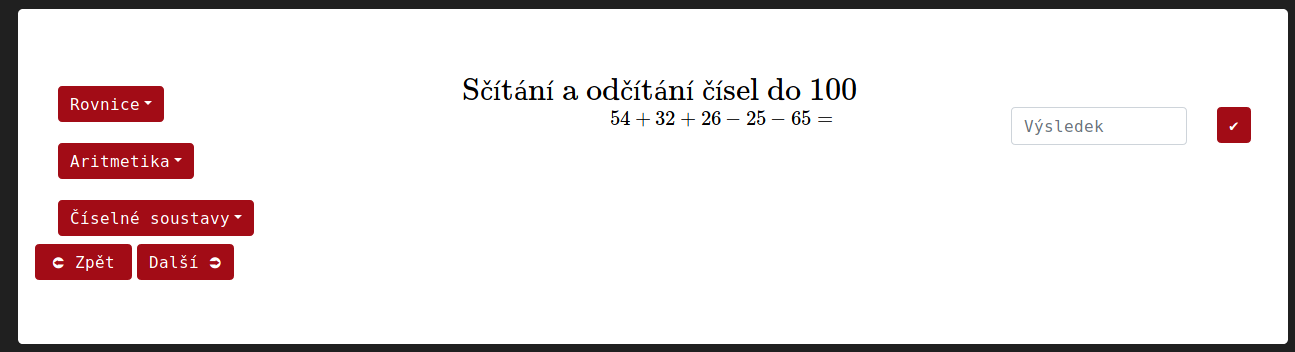
\includegraphics{../doc-images/WhiteBox.png}

Tato část je ohraničena dvěmi značkami:

\begin{Shaded}
\begin{Highlighting}[]
\KeywordTok{<template>}
\NormalTok{    ...}
\KeywordTok{</template>}
\end{Highlighting}
\end{Shaded}

V aplikaci je použit
\href{https://bootstrap-vue.js.org/docs}{bootstrap-vue}. Prosím,
zachovejte tento framework. Nejdůležitější značky jsou:

\begin{Shaded}
\begin{Highlighting}[]
\CommentTok{<!-- v sekci Layout and Grid System* -->}
\KeywordTok{<b-row>}
\NormalTok{    ...}
\KeywordTok{</b-row>}

\KeywordTok{<b-col}\OtherTok{ cols=}\StringTok{''}\KeywordTok{>}
\NormalTok{    ...}
\KeywordTok{</b-col>}

\CommentTok{<!-- v sekci Form** -->}
\KeywordTok{<b-form-input>}
\NormalTok{    ...}
\KeywordTok{</b-form-input>}
\end{Highlighting}
\end{Shaded}

*\href{https://bootstrap-vue.js.org/docs/components/layout}{Layout and
Grid System}\\
**\href{https://bootstrap-vue.js.org/docs/components/form}{Form}

\hypertarget{mathjax}{%
\subsection{Mathjax}\label{mathjax}}

Veškeré texty, které chcete vypsat v LATEXu musíte
\protect\hyperlink{Bind}{nabindovat} do tohoto komponentu:

\begin{Shaded}
\begin{Highlighting}[]
\KeywordTok{<vue-mathjax}\OtherTok{ :formula=}\StringTok{"var*"}\KeywordTok{/>}
\end{Highlighting}
\end{Shaded}

*vámi zvolená proměnná - specifikujete ji v sekci
\protect\hyperlink{data}{data}\\
Proměnná musí být v platném LATEXovém tvaru.\\
Začne "\$\$ a skončí \$\$".\\
Všechna zpětná lomítka \texttt{\textbackslash{}} musí být zdvojena.\\
Příklad takovéto proměnné:

\begin{Shaded}
\begin{Highlighting}[]
\NormalTok{discriminant}\OperatorTok{:} \StringTok{'\$\$x_\{1;2\} = \{-b }\SpecialCharTok{\textbackslash{}\textbackslash{}}\StringTok{pm }\SpecialCharTok{\textbackslash{}\textbackslash{}}\StringTok{sqrt\{b^2-4ac\} }\SpecialCharTok{\textbackslash{}\textbackslash{}}\StringTok{over 2a\}\$\$'}\OperatorTok{,}
\end{Highlighting}
\end{Shaded}

Bindovala by se tedy takto:

\begin{Shaded}
\begin{Highlighting}[]
\KeywordTok{<vue-mathjax}\OtherTok{ :formula=}\StringTok{"discriminant"}\KeywordTok{/>}
\end{Highlighting}
\end{Shaded}

Můžete ale také používat i tzv.
\protect\hyperlink{vuxfdvojuxe1ux159skuxe9-komponenty}{vývojářské
komponenty}:

\begin{Shaded}
\begin{Highlighting}[]
\KeywordTok{<nbsp>}
\NormalTok{    ...}
\KeywordTok{</nbsp>}

\KeywordTok{<hint-form>}
\NormalTok{    ...}
\KeywordTok{</hint-form>}

\CommentTok{<!-- A v neposlední řadě velmi důležitý komponent, který sjednocuje nadpisy}
\CommentTok{jednotlivých příkladů. -->}
\KeywordTok{<heading>}
\NormalTok{    ...}
\KeywordTok{</heading>}
\end{Highlighting}
\end{Shaded}

\textbf{Pozor! Je důležité všechny vývojařské komponenty správně
naimportovat (bude vysvětleno následovně).}

\hypertarget{import}{%
\section{Import}\label{import}}

Část komponentu, která mu říká, které další komponenty a soubory si musí
naimportovat je vkládána přímo za tuto značku:

\begin{Shaded}
\begin{Highlighting}[]
\KeywordTok{<script>}
\end{Highlighting}
\end{Shaded}

Pokud nepoužíváte
\href{https://github.com/kubajj/ComputatisDevelopmentProject}{vývojářský
projekt}, tak naimportujte následující:

\begin{Shaded}
\begin{Highlighting}[]
    \ImportTok{import} \OperatorTok{\{}\NormalTok{ bus }\OperatorTok{\}} \ImportTok{from} \StringTok{'./../../../main.js'}
    \ImportTok{import} \OperatorTok{\{}\NormalTok{ VueMathjax }\OperatorTok{\}} \ImportTok{from} \StringTok{'vue-mathjax'}
    \ImportTok{import}\NormalTok{ Heading }\ImportTok{from} \StringTok{'./../DevelopComponents/Heading.vue'}
    \ImportTok{import}\NormalTok{ CheckAlerts }\ImportTok{from} \StringTok{'./../DevelopComponents/CheckAlerts.vue'}
\end{Highlighting}
\end{Shaded}

Jsou to soubory nezbytné pro správný chod příkladu.

Obecně import probíhá následovně:

\begin{Shaded}
\begin{Highlighting}[]
\ImportTok{import}\NormalTok{ name}\OperatorTok{*} \ImportTok{from} \StringTok{'path**'}
\end{Highlighting}
\end{Shaded}

* název, který budete používat - \emph{ideálně stejný nebo podobný názvu
souboru, používá se CamelCase}\\
**relativní cesta k souboru

\hypertarget{vue}{%
\section{Vue}\label{vue}}

Tato část je vkládána přímo za importy. Po jejím ukončení ukončete i
script část pomocí \texttt{\textless{}/script\textgreater{}}\\

Začíná takto:

\begin{Shaded}
\begin{Highlighting}[]
    \ImportTok{export} \ImportTok{default} \OperatorTok{\{}
\end{Highlighting}
\end{Shaded}

Dále můžete specifikovat tyto části:

\begin{Shaded}
\begin{Highlighting}[]
    \AttributeTok{data}\NormalTok{() }\OperatorTok{\{}
        \ControlFlowTok{return} \OperatorTok{\{}
\NormalTok{            ...}
        \OperatorTok{\}}
    \OperatorTok{\},}
\NormalTok{    components}\OperatorTok{:} \OperatorTok{\{}
\NormalTok{        ...}
    \OperatorTok{\},}
\NormalTok{    methods}\OperatorTok{:} \OperatorTok{\{}
\NormalTok{        ...}
    \OperatorTok{\},}
\NormalTok{    computed}\OperatorTok{:} \OperatorTok{\{}
\NormalTok{        ...}
    \OperatorTok{\},}  
\end{Highlighting}
\end{Shaded}

Funkce těchto jednotlivých částí nyní rozeberu.\\

\textbf{Každou část ukončete složenou závorkou a čárkou.} \texttt{\},}

\hypertarget{data}{%
\subsection{Data}\label{data}}

V části data můžete specifikovat jednotlivé proměnné. Používá se
javascriptový zápis pro objekty:

\begin{Shaded}
\begin{Highlighting}[]
\NormalTok{name}\OperatorTok{*:}\NormalTok{ value}\OperatorTok{**,}
\end{Highlighting}
\end{Shaded}

*name = jméno proměnné\\
**value = hodnota proměnné \emph{Všechny řádky ukončujte čárkou.}\\
Více o javascriptových objektech naleznete
\href{https://www.w3schools.com/js/js_objects.asp}{zde}.

Na takto definované proměnné můžete odkazovat dvěma způsoby: 1.
\texttt{this.var*} 2. \texttt{this.\$data.var*}\\
*var = název proměnné\\
Pokud na ně odkazujete z HTML části, prefix \texttt{this.} se nepřidává
(ani \texttt{\$data.}).

\hypertarget{komponenty}{%
\subsection{Komponenty}\label{komponenty}}

V této části můžete (\emph{je to nutné pro jejich používání})
specifikovat názvy naimportovaných komponentů. Zápis takovéto
specifikace:

\begin{Shaded}
\begin{Highlighting}[]
\StringTok{'heading'}\OperatorTok{:}\NormalTok{ Heading}\OperatorTok{,}
\CommentTok{//tedy:}
\StringTok{'var-name*'}\OperatorTok{:}\NormalTok{ ImportedVarName}\OperatorTok{**,}
\end{Highlighting}
\end{Shaded}

* var-name -\textgreater{} název komponentu, který chcete používat v
HTML části\\
př.\texttt{\textquotesingle{}heading\textquotesingle{}} používá tzv.
kebab-case.

** ImportedVarName -\textgreater{} Název, kterým jste ho popsal v
Importu\\

\emph{Všechny řádky ukončujte čárkou.}

\hypertarget{vuxfdvojuxe1ux159skuxe9-komponenty}{%
\subsection{Vývojářské
komponenty}\label{vuxfdvojuxe1ux159skuxe9-komponenty}}

U každého komponentu zde specifikuji tzv.
\href{https://vuejs.org/v2/guide/components-props.html}{props} a funkci.
Props (\emph{properties}) jsou data, které nadřazený komponent
(\emph{parent}) posílá podřadným komponentům (\emph{child}).

\hypertarget{heading.vue}{%
\subsubsection{Heading.vue}\label{heading.vue}}

Props:\\
- head (\texttt{String})

\begin{Shaded}
\begin{Highlighting}[]
\NormalTok{props}\OperatorTok{:}\NormalTok{ [}\StringTok{'head'}\NormalTok{]}\OperatorTok{,}
\end{Highlighting}
\end{Shaded}

Funkce: Upraví vámi nabindovaný nadpis do LATEXového tvaru a tím z něj
vytvoří stylový nadpis, který vypadá jako všechno ostatní.\\
\emph{Používejte prosím značku
\texttt{\textbackslash{}\textbackslash{}text\ \{\}} pro zachování mezer}

\hypertarget{checkalerts.vue}{%
\subsubsection{CheckAlerts.vue}\label{checkalerts.vue}}

Props:\\
- checked (\texttt{String}) - možné hodnoty: - `right' - `wrong' -
result (převážně \texttt{Integer}, ale lze i \texttt{String})

\begin{Shaded}
\begin{Highlighting}[]
\NormalTok{props}\OperatorTok{:}\NormalTok{ [}\StringTok{'checked'}\OperatorTok{,} \StringTok{'result'}\NormalTok{]}\OperatorTok{,}
\end{Highlighting}
\end{Shaded}

Funkce: Zobrazí rámeček s hláškou \texttt{Správně} nebo \texttt{Špatně},
která ukáže i vámi specifikovaný správný výsledek (\emph{proto je nutné
ho uvést}).

\hypertarget{nbsp.vue}{%
\subsubsection{Nbsp.vue}\label{nbsp.vue}}

Props:\\
- num (\texttt{Integer}) - v intervalu \emph{\textless1;
5\textgreater{}}

\begin{Shaded}
\begin{Highlighting}[]
\NormalTok{props}\OperatorTok{:}\NormalTok{ [}\StringTok{'num'}\NormalTok{]}\OperatorTok{,}
\end{Highlighting}
\end{Shaded}

Funkce: Zobrazí vámi předepsaný počet \texttt{\&nbsp}
(\emph{non-breaking space}).

\hypertarget{hintformborder.vue}{%
\subsubsection{HintFormBorder.vue}\label{hintformborder.vue}}

Props:\\
- value (\texttt{String}) - correctResult (\texttt{String}) - správný
výsledek jednotlivých inputů - placeHolder (\texttt{String}) -
placeholder jednotlivých inputů

\begin{Shaded}
\begin{Highlighting}[]
\NormalTok{props}\OperatorTok{:} \OperatorTok{\{}
    \DataTypeTok{value}\OperatorTok{:} \OperatorTok{\{}
        \DataTypeTok{type}\OperatorTok{:}\NormalTok{ String}
    \OperatorTok{\},}
    \DataTypeTok{correctResult}\OperatorTok{:} \OperatorTok{\{}
        \DataTypeTok{type}\OperatorTok{:}\NormalTok{ String}
    \OperatorTok{\},}
    \DataTypeTok{placeHolder}\OperatorTok{:} \OperatorTok{\{}
        \DataTypeTok{type}\OperatorTok{:}\NormalTok{ String}
    \OperatorTok{\},}
\OperatorTok{\},}
\end{Highlighting}
\end{Shaded}

Funkce: Umožní vám vytvořit několik stejných inputformů. Mají tu
vlastnost, že když se rovná correctResult a input uživatele, tak jejich
okraj zezelená. V jiném případě je okraj červený. Jejich class pro
stylování je \texttt{class="inputWithBorder"}. Klasicky u nich funguje
zapisování do proměnných pomocí \texttt{v-model}.

V případě touhy po vytvoření vlastního vývojářského komponentu není
žádný problém. Vytvořte ho a následně pošlete pull-request.
\emph{Prosím, o specifikování názvu a přiložení části dokumentace v
syntaxu markdown.}

\hypertarget{metody}{%
\subsection{Metody}\label{metody}}

V této části můžete vytvořit jednotlivé metody, které lze volat v reakci
na akce uživatele. Zápis je dvojí podoby:

\begin{Shaded}
\begin{Highlighting}[]
\AttributeTok{genTask}\NormalTok{() }\OperatorTok{\{} 
    
\DataTypeTok{genTask}\OperatorTok{:} \KeywordTok{function}\NormalTok{() }\OperatorTok{\{}
\end{Highlighting}
\end{Shaded}

\begin{Shaded}
\begin{Highlighting}[]
    \CommentTok{//po složené závorce následuje obsah metody}
    \KeywordTok{this}\NormalTok{.}\AttributeTok{task} \OperatorTok{=} \StringTok{'$$ 1234 $$'}\OperatorTok{;}
\NormalTok{    \}}\OperatorTok{,}
\NormalTok{\}}\OperatorTok{,}
\end{Highlighting}
\end{Shaded}

Pokud je vaše metoda dlouhá, snažte se ji rozdělit na kratší metody.
Snadno je mezi sebou můžete volat pomocí prefixu \texttt{this.} společně
s názvem metody. \emph{Nezapomeňte na závorky.} př.
\texttt{this.number\ =\ this.randomNumber(1,\ 999);}

Pro vytvoření dočasných proměnných používejte \texttt{var}.\\
př. \texttt{var\ number\ =\ this.randomNumber(1,999);}\\
Jejich nevýhodou je, že je nelze volat z jiných metod.\\
Nemusíte je ale specifikovat v sekci \protect\hyperlink{data}{data}.

\textbf{V metodách a v computed ukončujete řádky středníkem
``\texttt{;}''.}

\hypertarget{uux17eiteux10dnuxe9-metody}{%
\subsection{Užitečné metody}\label{uux17eiteux10dnuxe9-metody}}

\hypertarget{random-number}{%
\subsubsection{Random Number}\label{random-number}}

Metoda, která vám vygeneruje náhodné číslo v uzavřeném intervalu mezi
čísly v závorce:

\begin{Shaded}
\begin{Highlighting}[]
\AttributeTok{randomNumber}\NormalTok{(min}\OperatorTok{,}\NormalTok{ max) }\OperatorTok{\{}\CommentTok{/*tato metoda generuje náhodné číslo (celé) z intervalu, }
\CommentTok{                        který je specifikován v závorkách*/}
    \ControlFlowTok{return} \VariableTok{Math}\NormalTok{.}\AttributeTok{floor}\NormalTok{(}\VariableTok{Math}\NormalTok{.}\AttributeTok{random}\NormalTok{() }\OperatorTok{*}\NormalTok{ (max }\OperatorTok{-}\NormalTok{ min }\OperatorTok{+} \DecValTok{1}\NormalTok{)) }\OperatorTok{+}\NormalTok{ min}\OperatorTok{;}
\OperatorTok{\},}
\end{Highlighting}
\end{Shaded}

\hypertarget{check}{%
\subsubsection{Check}\label{check}}

Umožní vám zkontrolovat výsledek uživatele:

\begin{Shaded}
\begin{Highlighting}[]
\AttributeTok{check}\NormalTok{() }\OperatorTok{\{}
    \ControlFlowTok{if}\NormalTok{ (}\KeywordTok{this}\NormalTok{.}\AttributeTok{checked} \OperatorTok{==} \StringTok{'right'}\NormalTok{) }\OperatorTok{\{} \CommentTok{/*pokud je výsledek, který uživatel odeslal }
\CommentTok{        správný, a uživatel znovu stlačí klávesu enter (nebo znovu potvrdí }
\CommentTok{        výsledek pomocí tlačítka), ukáže uživateli další příklad*/}
        \KeywordTok{this}\NormalTok{.}\AttributeTok{genTask}\NormalTok{()}\OperatorTok{;}
        \ControlFlowTok{return}\OperatorTok{;}
    \OperatorTok{\}}
    \ControlFlowTok{if}\NormalTok{ (}\KeywordTok{this}\NormalTok{.}\AttributeTok{usersResult} \OperatorTok{==} \KeywordTok{this}\NormalTok{.}\AttributeTok{result}\NormalTok{) }\OperatorTok{\{} \CommentTok{/*zkrontroluje, jestli je výsledek, }
\CommentTok{        který uživatel zadal, správný*/}
\CommentTok{        this.checked = 'right';}
\CommentTok{    \} else \{}
\CommentTok{        this.checked = 'wrong';}
\CommentTok{    \}}
\CommentTok{    document.getElementById("inputForm").value = '';}
\CommentTok{\},}
\end{Highlighting}
\end{Shaded}

Pokud nepoužívate
\href{https://github.com/kubajj/ComputatisDevelopmentProject}{vývojářský
projekt}, kde je již naimplementována, je nutné ji implementovat.

\hypertarget{grade}{%
\subsubsection{Grade}\label{grade}}

Umožní vám zjistit nejvyšší řád čísla:

\begin{Shaded}
\begin{Highlighting}[]
\AttributeTok{grade}\NormalTok{(givenNum) }\OperatorTok{\{}
    \ControlFlowTok{return} \VariableTok{Math}\NormalTok{.}\AttributeTok{ceil}\NormalTok{(}\VariableTok{Math}\NormalTok{.}\AttributeTok{log10}\NormalTok{(givenNum))}\OperatorTok{;}
\OperatorTok{\},}
\end{Highlighting}
\end{Shaded}

(\emph{Zaměnitelná s \texttt{*.length}.})

\hypertarget{reset-all}{%
\subsubsection{Reset All}\label{reset-all}}

Metoda, kterou doporučuji vytvořit, pokud potřebujete vymazat hodnotu
více proměnných naráz. př. užití:

\begin{Shaded}
\begin{Highlighting}[]
\AttributeTok{resetAll}\NormalTok{() }\OperatorTok{\{}
    \KeywordTok{this}\NormalTok{.}\AttributeTok{hinted} \OperatorTok{=} \KeywordTok{false}\OperatorTok{;}
    \KeywordTok{this}\NormalTok{.}\AttributeTok{checked} \OperatorTok{=} \StringTok{''}\OperatorTok{;}
    \KeywordTok{this}\NormalTok{.}\AttributeTok{hint} \OperatorTok{=} \StringTok{''}\OperatorTok{;}
    \KeywordTok{this}\NormalTok{.}\AttributeTok{comment} \OperatorTok{=} \StringTok{''}\OperatorTok{;}
    \KeywordTok{this}\NormalTok{.}\AttributeTok{correctCalculation} \OperatorTok{=}\NormalTok{ []}\OperatorTok{;}
    \ControlFlowTok{for}\NormalTok{ (}\KeywordTok{let}\NormalTok{ i }\OperatorTok{=} \DecValTok{0}\OperatorTok{;}\NormalTok{ i }\OperatorTok{<} \KeywordTok{this}\NormalTok{.}\VariableTok{resultsInputs}\NormalTok{.}\AttributeTok{length}\OperatorTok{;}\NormalTok{ i}\OperatorTok{++}\NormalTok{) }\OperatorTok{\{}\CommentTok{//vymaže hodnotu každého prvku pole                }
        \KeywordTok{this}\NormalTok{.}\VariableTok{$data}\NormalTok{.}\AttributeTok{resultsInputs}\NormalTok{[i] }\OperatorTok{=} \StringTok{''}\OperatorTok{;}
    \OperatorTok{\}}
    \KeywordTok{this}\NormalTok{.}\AttributeTok{specialHint} \OperatorTok{=} \KeywordTok{false}\OperatorTok{;}
    \KeywordTok{this}\NormalTok{.}\AttributeTok{placeHolders} \OperatorTok{=}\NormalTok{ []}\OperatorTok{;}
\OperatorTok{\},}
\end{Highlighting}
\end{Shaded}

\hypertarget{convert-number}{%
\subsubsection{Convert Number}\label{convert-number}}

Umí převádět čísla mezi jednotlivými číselnými soustavami:

\begin{Shaded}
\begin{Highlighting}[]
\AttributeTok{convertNumber}\NormalTok{(n}\OperatorTok{,}\NormalTok{ fromBase}\OperatorTok{,}\NormalTok{ toBase) }\OperatorTok{\{}
    \ControlFlowTok{if}\NormalTok{ (fromBase }\OperatorTok{===} \KeywordTok{void} \DecValTok{0}\NormalTok{) }\OperatorTok{\{}
\NormalTok{      fromBase }\OperatorTok{=} \DecValTok{10}\OperatorTok{;}
    \OperatorTok{\}}
    \ControlFlowTok{if}\NormalTok{ (toBase }\OperatorTok{===} \KeywordTok{void} \DecValTok{0}\NormalTok{) }\OperatorTok{\{}
\NormalTok{       toBase }\OperatorTok{=} \DecValTok{10}\OperatorTok{;}
    \OperatorTok{\}}
    \ControlFlowTok{return} \AttributeTok{parseInt}\NormalTok{(}\VariableTok{n}\NormalTok{.}\AttributeTok{toString}\NormalTok{()}\OperatorTok{,}\NormalTok{ fromBase).}\AttributeTok{toString}\NormalTok{(toBase)}\OperatorTok{;}
\OperatorTok{\},}
\end{Highlighting}
\end{Shaded}

\hypertarget{computed}{%
\subsection{Computed}\label{computed}}

Tato část vám umožňuje vytvářet proměnné, které budou výsledkem
metody.\\
\textbf{Je nutné ukončit je příkazem \texttt{return}.}\\
Zápis je stejný jako u metod, jen je v jiné části:

\begin{Shaded}
\begin{Highlighting}[]
\NormalTok{computed}\OperatorTok{:} \OperatorTok{\{}
    \AttributeTok{onePlusOne}\NormalTok{() }\OperatorTok{\{}
        \ControlFlowTok{return} \DecValTok{1} \OperatorTok{+} \DecValTok{1}\OperatorTok{;}
    \OperatorTok{\},}
\OperatorTok{\},}
\end{Highlighting}
\end{Shaded}

Lze z nich i klasicky volat jiné metody a také jiné computed
properties.\\
Více o \href{https://vuejs.org/v2/guide/computed.html}{computed
properties}.

\hypertarget{bind}{%
\subsection{Bind}\label{bind}}

Bindování znamená to, že z html části odkazujeme na nějakou proměnnou z
javascriptové/vue části. Děláme to pomocí dvou značek: 1.
\texttt{v-bind:var*}\\
2. \texttt{:var*}\\
* značkou var je míněn název proměnné, kterou chcete bindovat

\hypertarget{lifecycle-hooks}{%
\subsection{Lifecycle Hooks}\label{lifecycle-hooks}}

Toto je poslední druh, který lze použít v
\texttt{export\ default\ \{\}}. Jedná se o tyto značky:

\begin{Shaded}
\begin{Highlighting}[]
\AttributeTok{beforeCreate}\NormalTok{() }\OperatorTok{\{}
\NormalTok{    ...}
\OperatorTok{\},}
\AttributeTok{created}\NormalTok{() }\OperatorTok{\{}
\NormalTok{    ...}
\OperatorTok{\},}
\AttributeTok{beforeMount}\NormalTok{() }\OperatorTok{\{}
\NormalTok{    ...}
\OperatorTok{\},}
\AttributeTok{mounted}\NormalTok{() }\OperatorTok{\{}
\NormalTok{    ...}
\OperatorTok{\},}
\NormalTok{...}
\end{Highlighting}
\end{Shaded}

Všechny je můžete najít v tomto
\href{https://vuejs.org/v2/guide/instance.html\#Lifecycle-Diagram}{diagramu}.
Umožňují vám specifikovat, které metody se kdy spustí.

př. užití:

\begin{Shaded}
\begin{Highlighting}[]
\CommentTok{//Následující kód prosím zaimplementujte do svého hlavního komponentu. Bez něj je nepoužitelný.}
\AttributeTok{beforeMount}\NormalTok{() }\OperatorTok{\{}
    \KeywordTok{this}\NormalTok{.}\AttributeTok{genTask}\NormalTok{()}\OperatorTok{;}
\OperatorTok{\},}
\AttributeTok{mounted}\NormalTok{() }\OperatorTok{\{}
    \VariableTok{bus}\NormalTok{.}\AttributeTok{$on}\NormalTok{(}\StringTok{'next'}\OperatorTok{,} \KeywordTok{this}\NormalTok{.}\AttributeTok{genTask}\NormalTok{)}\OperatorTok{;}
\OperatorTok{\},}

\CommentTok{//Příklad jiného použítí:}
\AttributeTok{mounted}\NormalTok{() }\OperatorTok{\{}
    \KeywordTok{this}\NormalTok{.}\AttributeTok{resultsOfUnitInputs} \OperatorTok{=} \KeywordTok{this}\NormalTok{.}\VariableTok{correctUnit}\NormalTok{.}\AttributeTok{map}\NormalTok{(() }\KeywordTok{=>} \StringTok{''}\NormalTok{)}\OperatorTok{;}
    \KeywordTok{this}\NormalTok{.}\AttributeTok{resultsOfDecInputs} \OperatorTok{=} \KeywordTok{this}\NormalTok{.}\VariableTok{correctDec}\NormalTok{.}\AttributeTok{map}\NormalTok{(() }\KeywordTok{=>} \StringTok{''}\NormalTok{)}\OperatorTok{;}
    \KeywordTok{this}\NormalTok{.}\AttributeTok{resultsOfResInputs} \OperatorTok{=} \KeywordTok{this}\NormalTok{.}\VariableTok{correctResultSpaces}\NormalTok{.}\AttributeTok{map}\NormalTok{(() }\KeywordTok{=>} \StringTok{''}\NormalTok{)}\OperatorTok{;}
\OperatorTok{\},} 
\end{Highlighting}
\end{Shaded}

\textbf{Vue část se uzavírá značkou
\texttt{\textless{}/script\textgreater{}}.}

\hypertarget{css}{%
\section{CSS}\label{css}}

Pro úpravu vzhledu se nepoužívají žádné externí soubory.\\
Použijte kaskádové styly mezi značkami
\texttt{\textless{}style\textgreater{}} a
\texttt{\textless{}/style\textgreater{}}.

\hypertarget{zveux159ejnux11bnuxed-vaux161eho-komponentu}{%
\section{Zveřejnění vašeho
komponentu}\label{zveux159ejnux11bnuxed-vaux161eho-komponentu}}

Vytvořte pull-request, ve kterém popíšete vámi vytvořený příklad a
pojmenujete ho.\\
Název i kód musí být zkontrolován, proto prosím o stručný popis toho, co
váš kód dělá.\\
Následně bude zařazen do příslušné tématické složky a zveřejněn.

\hypertarget{faq}{%
\section{FAQ}\label{faq}}

\emph{Nemáte nějaký videotutoriál na Vue.js?}\\
\href{https://www.youtube.com/playlist?list=PL4cUxeGkcC9gQcYgjhBoeQH7wiAyZNrYa}{www.youtube.com/playlist?list=PL4cUxeGkcC9gQcYgjhBoeQH7wiAyZNrYa}

\emph{Jak posílat data z child komponent na parent?}\\
Pomocí
\href{https://vuejs.org/v2/guide/components.html\#Listening-to-Child-Components-Events}{\texttt{\$emit}}.

\end{document}
